%%%%%
%%Title: HiPi+Bus V0.2 Chapter 3 Section 3
%%Creator: Ando Ki
%%CreationDate: April 1992
%%FileName: sec3
%%RelatedFile: ch3
%%%%%
%\documentstyle[doublespace,a4wide]{hbook}
%\setstretch{1.2}
%\pagestyle{headings}
%\begin{document}
%\pagenumbering{arabic}
%\setcounter{chapter}{1}
%
\section{데이터 전송}
버스는 기본적으로 데이터 이동의 통로이며 이러한 데이터 이동은 버스 상에 장착된 
보드들 사이에서 이루어진다. 이들 데이터 이동에 참여하는 보드는 특정 시간에 어떤 일을 하느냐에 따라
RQ(ReQuester)와 RP(ResPonder)로 구분한다.
RQ는 데이터 이동에 능동적으로 참여하며 데이터 전송을 시작하는 기능을 수행중인 보드이며,
RP는 데이터 이동에 수동적으로 참여하며 RQ의 데이터 전송 요청에 응답하는 보드이다.
일반적으로 RQ는 프로세서 보드가 수행하는 기능에 해당하며, RP는 메모리 보드가 수행하는 기능에 해당한다.
그러나 프로세서 보드가 RP로도 동작한다면 RP라고 할 수 있다. \\
데이터 전송(data transfer)은 버스 동작(bus transaction)으로 수행되며,
버스 동작은 기본 사이클(basic cycle)로 구성된다.
데이터 전송은 데이터 이동의 관점에서 읽기, 쓰기, 그리고 무효화로 구분된다.
읽기는 RQ가 특정 주소의 데이터를 필요로 하여 요청하는 전송이며,
쓰기는 RQ가 특정 주소의 데이터를 공급하는 전송이다.
무효화는 데이터 이동이 없고 특정 주소에 대한 특별한 의미를 전달할 때 사용된다.\\
버스 동작은 데이터 전송을 위해 진행되는 일련의 동작으로 RQ에 의해 시작되며
기본 사이클로 이루어 진다. 특히 진행되는 버스 동작은 완전하게 종결되는 경우도
있지만 진행 중에 중단되는 경우도 있다. 완전하게 종결되는 경우 데이터 이동이
완벽하게 이루어진 경우이며 중단된 경우 해당 데이터 전송을 위해 처음부터 다시
버스 동작을 시도하여야 한다. \\
%
\subsection{데이터 전송의 기본 사이클}
기본 사이클은 분리될 수 없는 일정한 순서로 진행되는 단계(phase)로 구성되며,
각 단계는 한개의 버스 클럭 주기(bus clock period)가 소요된다.
기본 사이클에는 어드레스 기본 사이클(address basic cycle),
단일 전송 데이터 기본 사이클(data basic cycle), 단일 전송 어드레스 데이터 기본 사이클(address
data basic cycle), 블록 전송 데이터 기본 사이클(block data basic cycle),
그리고 블록 전송 어드레스 데이터 기본 사이클(block address data basic cycle)이 있다. \\
어드레스 기본 사이클은 어드레스와 해당 어드레스에 관련된 정보의 이동 또는 전달에 사용된다.
이 어드레스 기본 사이클은 반드시 RQ에 의해 수행된다.
단일 전송 데이터 기본 사이클과 블록 전송 데이터 기본 사이클은
어드레스 기본 사이클에 의해 요청된 데이터의 전달에 사용되며,
반드시 RP에 의해 수행된다.
단일 전송 어드레스 데이터 기본 사이클과 블록 전송 어드레스 데이터 기본 사이클은
어드레스와 해당 어드레스의 데이터를 동시에 이동 또는 전달할 때 사용되며,
반드시 RQ에 의해 수행된다.
%
\subsubsection{어드레스 기본 사이클}
어드레스 정보(어드레스와 이에 관련된 정보들)를 전달할 때 사용하는 기본 사이클이며
반드시 어드레스 중재 과정을 거친 후에
수행되어야 한다. 이 기본 사이클은 3개의 단계로 구성되며 각 단계는 연속적이다.
어드레스 중재를 수행하여 어드레스 버스 사용권을 획득한 바로 다음 버스 클럭 주기에 어드레스 기본 사이클의
단계 0(phase 0)가 시작된다. RQ는 단계 0에서는 어드레스 정보를
어드레스 버스에 구동한다. 단계 1에서는 각 RP들이 단계 0에 전달된 어드레스 정보를 번역하여
필요한 동작을 준비한다. 이때 RQ는 그냥 기다린다.
단계 2에서는 단계 1에서 결정된 RP가 전달받은 어드레스 정보에 대한 응답(어드레스 응답)을 구동하며,
RQ는 이 어드레스 응답을 받아 수행한 어드레스 기본 사이클의 완성 여부를 판단한다. \\
어드레스 기본 사이클에 의해 수행되는 버스 동작이 읽기인 경우 RQ는 RP로부터 데이터가
전달되어 오기를 기다리게 되고, 선택된 RP는 요청된 데이터를 전달하기 위해 데이터 기본 사이클을
수행해야 된다.
%\input{ch3/TBL/address-basic}
\begin{figure}[hp]
   \centerline{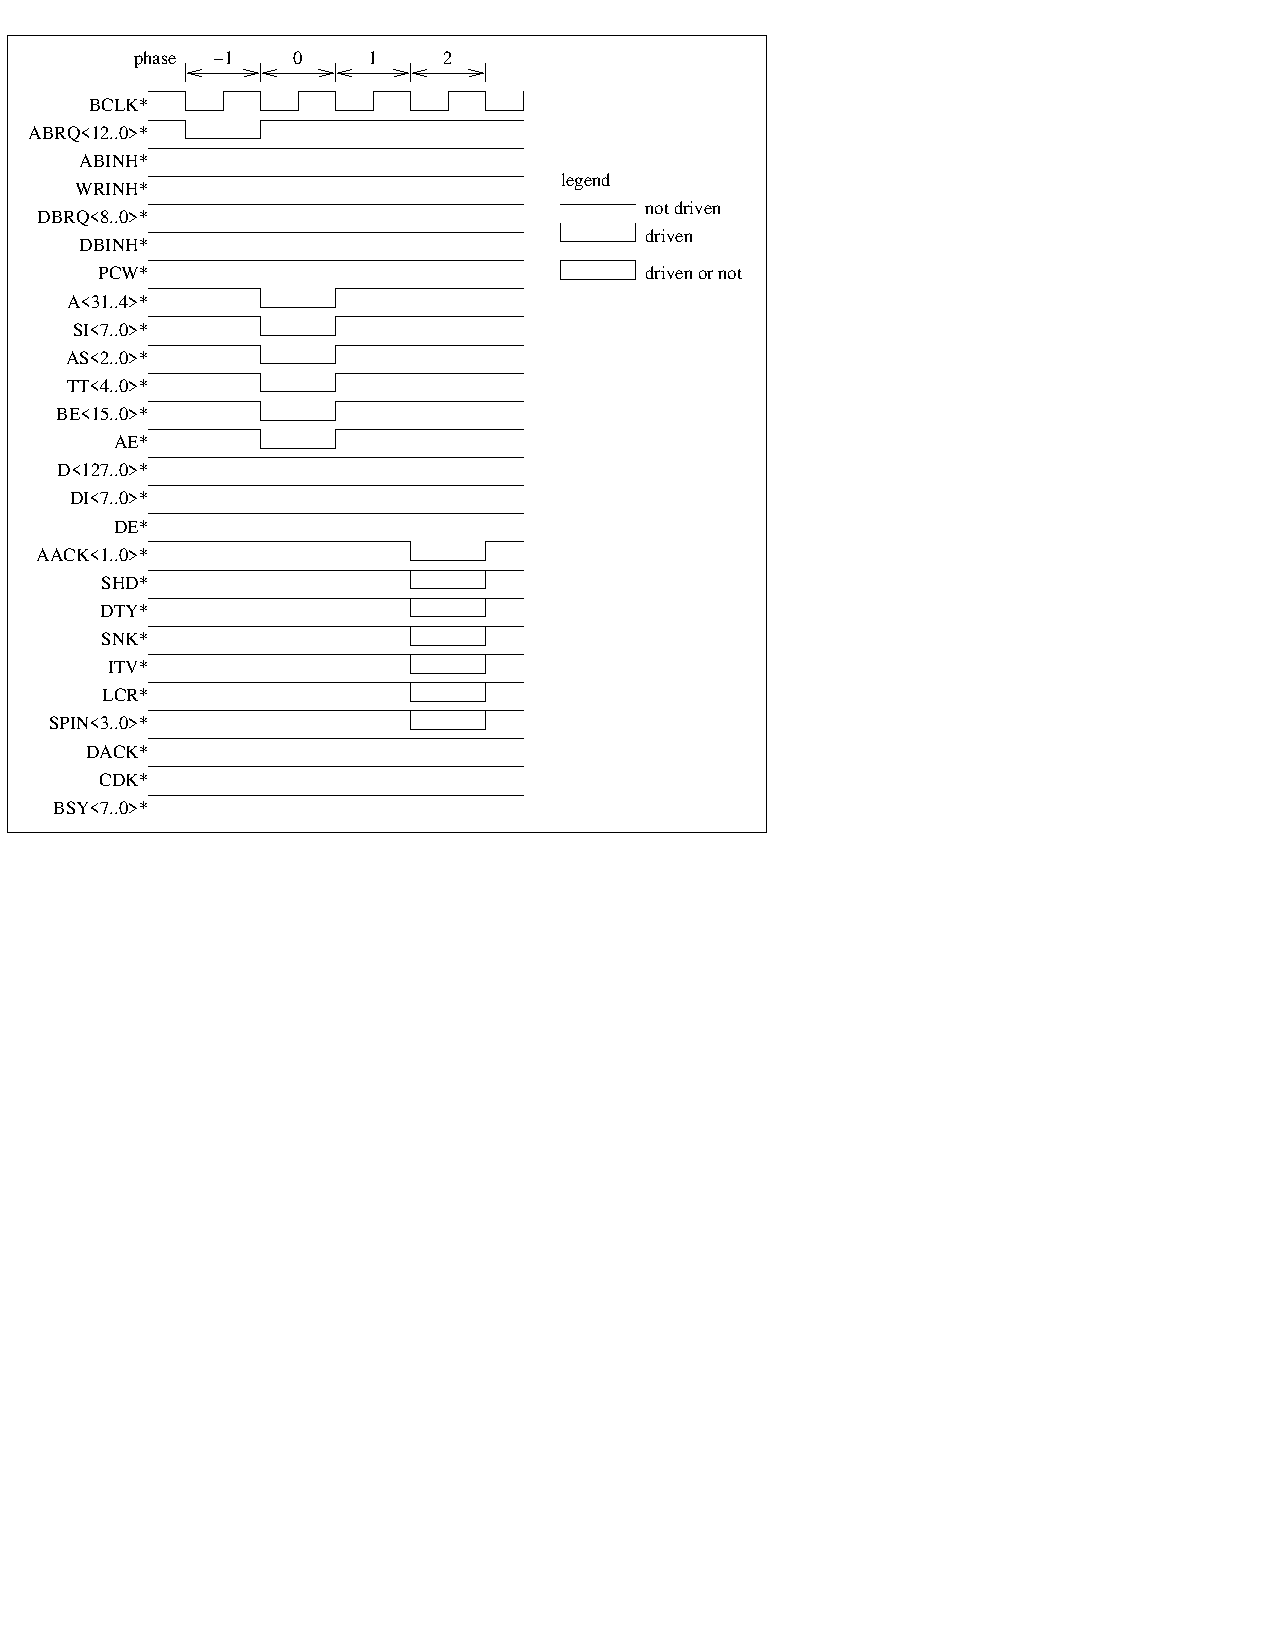
\includegraphics{ch3/FIG/single-add-basic.jpg}}
   \caption{어드레스 기본 사이클}\label{figure:single-add-basic}
\end{figure}
\begin{itemize}
	\item 어드레스 버스 중재 주기 - 단계 -1 (phase -1)\\
	어드레스 버스에 해당 어드레스를 구동하기에 앞서 수행하는 어드레스 버스 중재 주기.
	\item 어드레스 기본 주기 - 단계 0 (phase 0)\\
	중재 버스를 통하여 버스 사용허가를 받은 RQ가 한 버스 클럭 주기 동안 
	버스 상에 어드레스와 관련한 정보를 전송한다.
	32 비트의 어드레스, 어드레스 영역, 전송 형태, 바이트 마스크, RQ의 슬롯과
	채널 어드레스등과 각 신호의 패리티가 전송된다.
	이 주기 동안 사용되는 신호는 A$<$31..4$>$*, AP$<$3..0$>$*,
	AS$<$2..0$>$*, TT$<$4..0$>$*, STP*,
	BE$<$15..0$>$*, BEP$<$1..0$>$*,
	SI$<$7..0$>$*, SIP*, AE* 등이다.
	RP들은 이 단계의 끝 부분에서 어드레스 버스에 실린 신호를 모두 저장한다. \\
	캐쉬를 갖는 RQ 들도 이 단계의 끝 부분에서 어드레스 버스에 실린 신호를 모두 저장한다.
%
	\item 어드레스 기본 주기 - 단계 1 (phase 1)\\
	이 단계는 버스 상의 신호의 구동은 없다.
	단계 0에서 어드레스 버스를 구동했던 RQ는 다음 동작을 준비한다.
	단계 0에서 전송된 어드레스 등의 정보를 받은 RP들은 내부적으로  단계 2를 위한 동작이 수행된다.
	우선 RP는 각 정보의 패리티 에러 확인을 한다. 패리티 에러가 발견되지 않은 경우
	RP들은 저장한 어드레스를 번역하여 전송된 어드레스가 자신의 영역을 지정했는지를 확인한다.
	선택된 하나의 RP만 자신의 상태를 점검하여 단계 2에서 전송할 신호의 내용을 준비한다. \\
	캐쉬를 갖는 RQ들은 캐쉬 동일성 유지를 위한 동작을 내부적으로 수행한다.
%
	\item 어드레스 기본 주기 - 단계 2 (phase 2)\\
	단계 2에서는 어드레스에 의해 선정된 한 RP가 단계 0에서 전송된 정보들에
	대한 응답을 버스 상에 구동한다. 
	이때 사용되는 신호는 AACK$<$1..0$>$* 이고,
	단계 0에서 어드레스를 전송했던 RQ는 이 정보를 받아서 저장한다.
	이 단계 후의 RP와 RQ의 내부적인 동작은 기본 주기에서 규정하지 않는다.
	단계 1에서 패리티 에러가 검출된 경우 RP는 신호를 구동하지 않는다. \\
	캐쉬를 갖는 RQ들은 단계 0에서 저장한 어드레스에 대해 
	캐쉬 동일성 유지 동작을 수행함에 있어서 문제가 발생하면 SNK* 신호를 구동한다.
	또는 캐쉬 동일성 유지 동작에 필요한 SHD*, DTY*, ITV* 신호를
	구동한다.
\end{itemize}
%
\subsubsection{단일 전송 데이터 기본 사이클}
이미 수행된 어드레스 기본 사이클에서 데이터 요청이 발생한 경우 RP가 해당 어드레스의 데이터를
RQ로 전달할 때 사용하며 반드시 데이터 버스중재 과정을 거친 후에 수행된다.
데이터 버스 중재를 수행하여 데이터 버스 사용권을 획득한 바로 다음 버스 클럭 주기에
데이터 기본 사이클이 수행된다.
%\input{ch3/TBL/data-basic}
\begin{figure}[hp]
   \centerline{\includegraphics{ch3/FIG/single-data-basic.jpg}}
   \caption{데이터 기본 사이클}\label{figure:single-data-basic}
\end{figure}
\begin{itemize}
	\item 데이터 버스 중재 주기 - 단계 -1 (phase -1)\\
	데이터 버스에 해당 데이터를 구동하기에 앞서 수행하는 데이터 버스 중재 동작.
%
	\item 데이터 기본 주기 - 단계 0 (phase 0)\\
	데이터 중재 버스를 통하여 데이터 전송 버스의 사용 허가를 받은 RP가
	데이터 전송 버스의 신호들을 구동한다.
	구동되는 버스의 신호는 D$<$127..0$>$*, DP$<$15..0$>$*,
	DI$<$7..0$>$*, DIP*, DE* 등이다.
	데이터 신호는 어드레스 기본 주기에 의해 전송된 영역에 해당되는 데이터가 구동되고,
	종착점 신호(DI$<$7..0$>$*)는 전송하는 데이터를 요청했던
	RQ의 시발점 신호(SI$<$7..0$>$*)를 구동한다.
	어드레스 주기를 통하여 RP로 데이터 요청을 한 RQ들(2개 이상이 될 수 있음)은
	데이터 버스의 신호를 저장한다.
%
	\item 데이터 기본 주기 - 단계 1 (phase 1)\\
	단계 0에서 데이터 버스를 구동했던 RP는 다음 동작을 준비한다.
	단계 0에서 전송된 데이터 등의 정보를 받은 RQ는 내부적으로  단계 2를 위한 동작이 수행된다.
	우선 RQ들은 내부적으로 전송된 정보 들의 패리티 에러의 확인을 한다.
	에러가 발견되지 않으며, 종착점 신호를 자신의 슬롯 어드레스와 비교하여
	전송된 데이터가 자신이 요청한 것인지를 확인하게 된다.
	자신의 데이터가 아니면 데이터의 저장을 무효화한다.
%
	\item 데이터 기본 주기 - 단계 2 (phase 2)\\
	단계 1에서 전송된 정보 중에 패리티 에러가 발견되면 
	DACK*를 구동하지 않고, 패리티 에러가 없으면 DACK*를 구동하여 RP로부터 전송된
	데이터를 RQ가 잘 받았음을 알린다.
	특히 해당 데이터에서 패리티 에러가 발견된 경우 RQ는 그 데이터 전송을 있게 한 어드레스 전송까지 무효화하고,
	어드레스 기본 주기부터 재시도한다.
\end{itemize}
%
\subsubsection{블록 전송 데이터 기본 사이클}
이미 수행된 어드레스 기본 사이클에서 데이터 요청이 있은 경우 RP가 해당 어드레스의 데이터를
RQ로 전달할 때 사용하며 반드시 데이터 중재 과정을 거친 후에 수행된다.
데이터 중재를 수행하여 데이터 버스 사용권을 획득한 바로 다음 버스 클럭 주기에
데이터 기본 사이클이 수행된다.
%\input{ch3/TBL/data-basic}
\begin{figure}[hp]
   \centerline{\includegraphics{ch3/FIG/block-data-basic.jpg}}
   \caption{블록 전송 데이터 기본 사이클}\label{figure:block-data-basic}
\end{figure}
\begin{itemize}
	\item 블록 전송 데이터 버스 중재 주기 - 단계 -1 (phase -1)\\
	데이터 버스에 해당 데이터를 구동하기에 앞서 수행하는 데이터 버스 중재 동작. \\
	블록 전송 어드레스 데이터 기본 주기의 데이터 구동과 충돌을 방지하기 위해
	WRINH* 신호를 구동한다.
%
	\item 블록 전송 데이터 기본 주기 - 단계 0 (phase 0)\\
	데이터 중재 버스를 통하여 데이터 전송 버스의 사용 허가를 받은 RP가
	데이터 전송 버스의 신호들을 구동한다.
	구동되는 버스의 신호는 D$<$127..0$>$*, DP$<$15..0$>$*,
	DI$<$7..0$>$*, DIP*, DE* 등이다.
	데이터 신호는 어드레스 기본 주기에 의해 전송된 영역에 해당되는 데이터가 구동되고,
	종착점 신호(DI$<$7..0$>$*)는 전송하는 데이터를 요청했던
	RQ의 시발점 신호(SI$<$7..0$>$*)를 구동한다.
	어드레스 주기를 통하여 RP로 데이터 요청을 RQ는
	데이터 버스의 신호를 저장한다. \\
	블록 전송 어드레스 데이터 기본 주기의 데이터 구동에 충돌을 방지하기 위해
	WRINH* 신호를 구동한다.
	다른 블록 전송 데이터 기본 주기의 데이터 구동과 충돌을 방지하기 위해
	DBINH* 신호를 구동한다.
%
	\item 블록 전송 데이터 기본 주기 - 단계 1 (phase 1)\\
	데이터 전송 버스의 신호들을 구동한다.
	구동되는 버스의 신호는 D$<$127..0$>$*, DP$<$15..0$>$*,
	DI$<$7..0$>$*, DIP*, DE* 등이다.
	데이터 신호는 어드레스 기본 주기에 의해 전송된 영역에 해당되는 데이터가 구동되고,
	종착점 신호(DI$<$7..0$>$*)는 전송하는 데이터를 요청했던
	RQ의 시발점 신호(SI$<$7..0$>$*)를 구동한다.
	어드레스 주기를 통하여 RP로 데이터를 요청한 RQ는
	데이터 버스의 신호를 저장한다. \\
	단계 0에서 데이터 버스를 구동했던 RP는 다음 동작을 준비한다.
	단계 0에서 전송된 데이터등의 정보를 받은 RP들은 내부적으로  단계 2를 위한 동작을 수행한다.
	우선 RQ들은 내부적으로 전송된 정보들의 패리티 에러의 유무를 확인한다.
	에러가 발견되지 않으며, 종착점 신호를 자신의 슬롯 어드레스와 비교하여
	전송된 데이터가 자신이 요청한 것인지를 확인하게 된다.
	자신의 데이터가 아니면 데이터의 저장을 무효화한다. \\
	블록 전송 어드레스 데이터 기본 주기의 데이터 구동에 충돌을 방지하기 위해
	WRINH* 신호를 구동한다.
	다른 블록 전송 데이터 기본 주기의 데이터 구동과 충돌을 방지하기 위해
	DBINH* 신호를 구동한다.
%
	\item 블록 전송 데이터 기본 주기 - 단계 2 (phase 2)\\
	데이터 전송 버스의 신호들을 구동한다.
	구동되는 버스의 신호는 D$<$127..0$>$*, DP$<$15..0$>$*,
	DI$<$7..0$>$*, DIP*, DE* 등이다.
	데이터 신호는 어드레스 기본 주기에 의해 전송된 영역에 해당되는 데이터가 구동되고,
	종착점 신호(DI$<$7..0$>$*)는 전송하는 데이터를 요청했던
	RQ의 시발점 신호(SI$<$7..0$>$*)를 구동한다.
	어드레스 주기를 통하여 RP로 데이터를 요청한 RQ는
	데이터 버스의 신호를 저장한다. \\
	단계 0에서 전송된 정보 중에 패리티 에러가 발견되면 
	DACK*를 구동하지 않고, 패리티 에러가 없으면 DACK*를 구동하여 RP로부터 전송된
	데이터를 RQ가 잘 받았음을 알린다.
	특히 해당 데이터에서 패리티 에러가 발견된 경우 RQ는 어드레스 기본 주기부터 재시도 한다. \\
	다른 블록 전송 데이터 기본 주기의 데이터 구동과 충돌을 방지하기 위해
	DBINH* 신호를 구동한다.
%
	\item 블록 전송 데이터 기본 주기 - 단계 3 (phase 3)\\
	데이터 전송 버스의 신호들을 구동한다.
	구동되는 버스의 신호는 D$<$127..0$>$*, DP$<$15..0$>$*,
	DI$<$7..0$>$*, DIP*, DE* 등이다.
	데이터 신호는 어드레스 기본 주기에 의해 전송된 영역에 해당되는 데이터가 구동되고,
	종착점 신호(DI$<$7..0$>$*)는 전송하는 데이터를 요청했던
	RQ의 시발점 신호(SI$<$7..0$>$*)를 구동한다.
	어드레스 주기를 통하여 RP로 데이터를 요청한 RQ는
	데이터 버스의 신호를 저장한다. \\
	단계 1에서 전송된 정보 중에 패리티 에러가 발견되면 
	DACK*를 구동하지 않고, 패리티 에러가 없으면 DACK*를 구동하여 RP로부터 전송된
	데이터를 RQ가 잘 받았음을 알린다.
	특히 해당 데이터에서 패리티 에러가 발견된 경우 RQ는 그 데이터 전송을 있게 한 어드레스 전송까지 무효화하고,
	어드레스 기본 주기부터 재시도한다.
	\item 블록 전송 데이터 기본 주기 - 단계 4 (phase 4)\\
	단계 2에서 전송된 정보 중에 패리티 에러가 발견되면 
	DACK*를 구동하지 않고, 패리티 에러가 없으면 DACK*를 구동하여 RP로부터 전송된
	데이터를 RQ가 잘 받았음을 알린다.
	특히 해당 데이터에서 패리티 에러가 발견된 경우 RQ는
	어드레스 기본 주기부터 재시도한다.
	\item 블록 전송 데이터 기본 주기 - 단계 5 (phase 5)\\
	단계 3에서 전송된 정보 중에 패리티 에러가 발견되면 
	DACK*를 구동하지 않고, 패리티 에러가 없으면 DACK*를 구동하여 RP로부터 전송된
	데이터를 RQ가 잘 받았음을 알린다.
	특히 해당 데이터에서 패리티 에러가 발견된 경우 RQ는
	어드레스 기본 주기부터 재시도한다.
\end{itemize}
%
\subsubsection{단일 전송 어드레스-데이터 기본 사이클}
어드레스 정보(어드레스와 이에 관련된 정보들)와 데이터 정보(데이터와 이에 관견된 정보들)를
동시에 전달할 때 사용하는
기본 사이클이며 반드시 어드레스 중재 과정을 거친 후에 수행되어야 한다.
이 기본 사이클은 4개의 단계로 구성되며 각 단계는 연속적이다.
어드레스 중재를 수행하여 어드레스 버스 사용권을 획득한 바로 다음 버스 클럭 주기에 어드레스-데이터 기본 사이클의
단계 0(phase 0)가 시작된다. RQ는 단계 0에서 어드레스 정보를
어드레스 버스에 구동한다. 단계 1에서는 각 RP들이 단계 0에 전달된 어드레스 정보를 번역하여
필요한 동작을 준비한다. 이때 RQ는 데이터 정보를 데이터 버스에 구동한다.
단계 2에서는 단계 1에서 결정된 RP가 전달받은 어드레스 정보에 대한 응답(어드레스 응답)을 구동하며,
동시에 단계 1에서 전달된 데이터를 점검한다.
단계 3에서는 RP가 단계 1에서 전달받은 데이터에 대한 데이터 응답을 구동한다.
RQ는 단계 2에 전달받은 어드레스 응답과 단계 3에 전달받은 데이터 응답에 의해
수행한 어드레스-데이터 기본 사이클의 완성 여부를 판단한다.
%\input{ch3/TBL/add-data-basic}
\begin{figure}[hp]
   \centerline{\includegraphics{ch3/FIG/single-add-data-basic.jpg}}
   \caption{어드레스 데이터 기본 사이클}\label{figure:single-add-data-basic}
\end{figure}
\begin{itemize}
	\item 단일 전송 어드레스 버스 중재 주기 - 단계 -1 (phase -1)\\
	어드레스 버스에 해당 어드레스를 구동하기에 앞서 수행하는 어드레스 버스 중재 동작.
	\item 단일 전송 어드레스 데이터 기본 주기 - 단계 0 (phase 0)\\
	중재 버스를 통하여 버스 사용허가를 받은 RQ가 한 버스 클럭 주기 동안 
	버스 상에 어드레스와 관련한 정보를 전송한다.
	32 비트의 어드레스, 어드레스 영역, 전송 형태, 바이트 마스크, RQ의 슬롯과
 	채널 어드레스등과 각 신호의 패리티가 전송된다.
	이 주기 동안 사용되는 신호는 A$<$31..4$>$*, AP$<$3..0$>$*,
	AS$<$2..0$>$*, TT$<$4..0$>$*, STP*,
	BE$<$15..0$>$*, BEP$<$1..0$>$*,
	SI$<$7..0$>$*, SIP*, AE* 등이다.
	RP들은 이 단계의 끝 부분에서 어드레스 버스에 실린 신호를 모두 저장한다. \\
	캐쉬를 갖는 RQ들도 이 단계의 끝 부분에서 어드레스 버스에 실린 신호를 모두 저장한다. \\
	데이터 기본주기와의 데이터 충돌을 방지하기 위해 DBINH* 신호를 구동한다.
%
	\item 단일 전송 어드레스 데이터 기본 주기 - 단계 1 (phase 1)\\
	단계 0를 구동한 RQ가 계속해서 데이터 버스를 구동한다.
	이 단계에서 구동되는 신호선은 D$<$127..0$>$*,
	DP$<$15..0$>$*, DI$<$7..0$>$*, DIP*, DE*등이다.
	데이터 기본 주기와는 달리 별도의 데이터 중재 과정이 없다.\\
	RP들은 단계 0에서 저장한 어드레스 버스의 정보들의 에러 확인과 번역을 수행한다.
	또한 단계 1의 부분에서는 RQ로부터 오는 데이터를 저장한다. \\
	캐쉬를 갖는 RQ들은 캐쉬 동일성 유지를 위한 동작을 내부적으로 수행한다.
%
	\item 단일 전송 어드레스 데이터 기본 주기 - 단계 2 (phase 2)\\
	단계 2에서는 어드레스에 의해 선정된 한 RP가 단계 0에서 전송된 정보들에
	대한 응답을 버스 상에 구동하고 단계 1에서 받은 데이터의 패리티 에러를 확인한다.
	이때 사용되는 신호는 AACK$<$1..0$>$* 이고,
	만약 단계 0에서 전송된 정보에 에러가 검출될 경우 신호 구동과 데이터 패리티 확인을
	수행하지 않는다. \\
	캐쉬를 갖는 RQ 들이 단계 0에서 저장한 어드레스에 대한 
	캐쉬 동일성 유지 동작을 수행함에 있어서 문제가 발생하면 SNK* 신호를 구동한다.
	단계 0를 수행했던 RQ는 어드레스 상태 신호를 저장한다. \\
%
	\item 단일 전송 어드레스 데이터 기본 주기 - 단계 3 (phase 3)\\
	단계 1에서 전송된 데이터를 받은 RP가 RQ로 응답하는 단계이다.
	데이터의 에러 유무를 보고한다. 이때 사용하는 신호선은 DACK*이다.
	단계 2의 응답에서 어드레스를 정상적으로 접수하지 못했다는 반응이 있었을 경우
	이 단계의 응답은 의미가 없다. \\
	RQ는 데이터 응답을 저장한다. \\
\end{itemize}
%
\subsubsection{블록 전송 어드레스-데이터 기본 사이클}
어드레스 정보(어드레스와 이에 관련된 정보들)와 데이터 정보(데이터와 이에 관견된 정보들)를
동시에 전달할 때 사용하는
기본 사이클이며 반드시 어드레스 중재 과정을 거친 후에 수행되어야 한다.
이 기본 사이클은 4개의 단계로 구성되며 각 단계는 연속적이다.
어드레스 중재를 수행하여 어드레스 버스 사용권을 획득한 바로 다음 버스 클럭 주기에 어드레스-데이터 기본 사이클의
단계 0(phase 0)가 시작된다. RQ는 단계 0에서는 어드레스 정보를
어드레스 버스에 구동한다. 단계 1에서는 각 RP들이 단계 0에 전달된 어드레스 정보를 번역하여
필요한 동작을 준비한다. 이때 RQ는 데이터 정보를 데이터 버스에 구동한다.
단계 2에서는 단계 0에서 결정된 RP가 전달받은 어드레스 정보에 대한 응답(어드레스 응답)을 구동하며,
동시에 단계 0에서 전달된 데이터를 점검한다.
단계 3에서는 RP가 단계 1에서 전달받은 데이터에 대한 데이터 응답을 구동한다.
RQ는 단계 2에 전달받은 어드레스 응답과 단계 3에 전달받은 데이터 응답에 의해
수행한 어드레스-데이터 기본 사이클의 완성 여부를 판단한다.
%\input{ch3/TBL/add-data-basic}
\begin{figure}[hp]
   \centerline{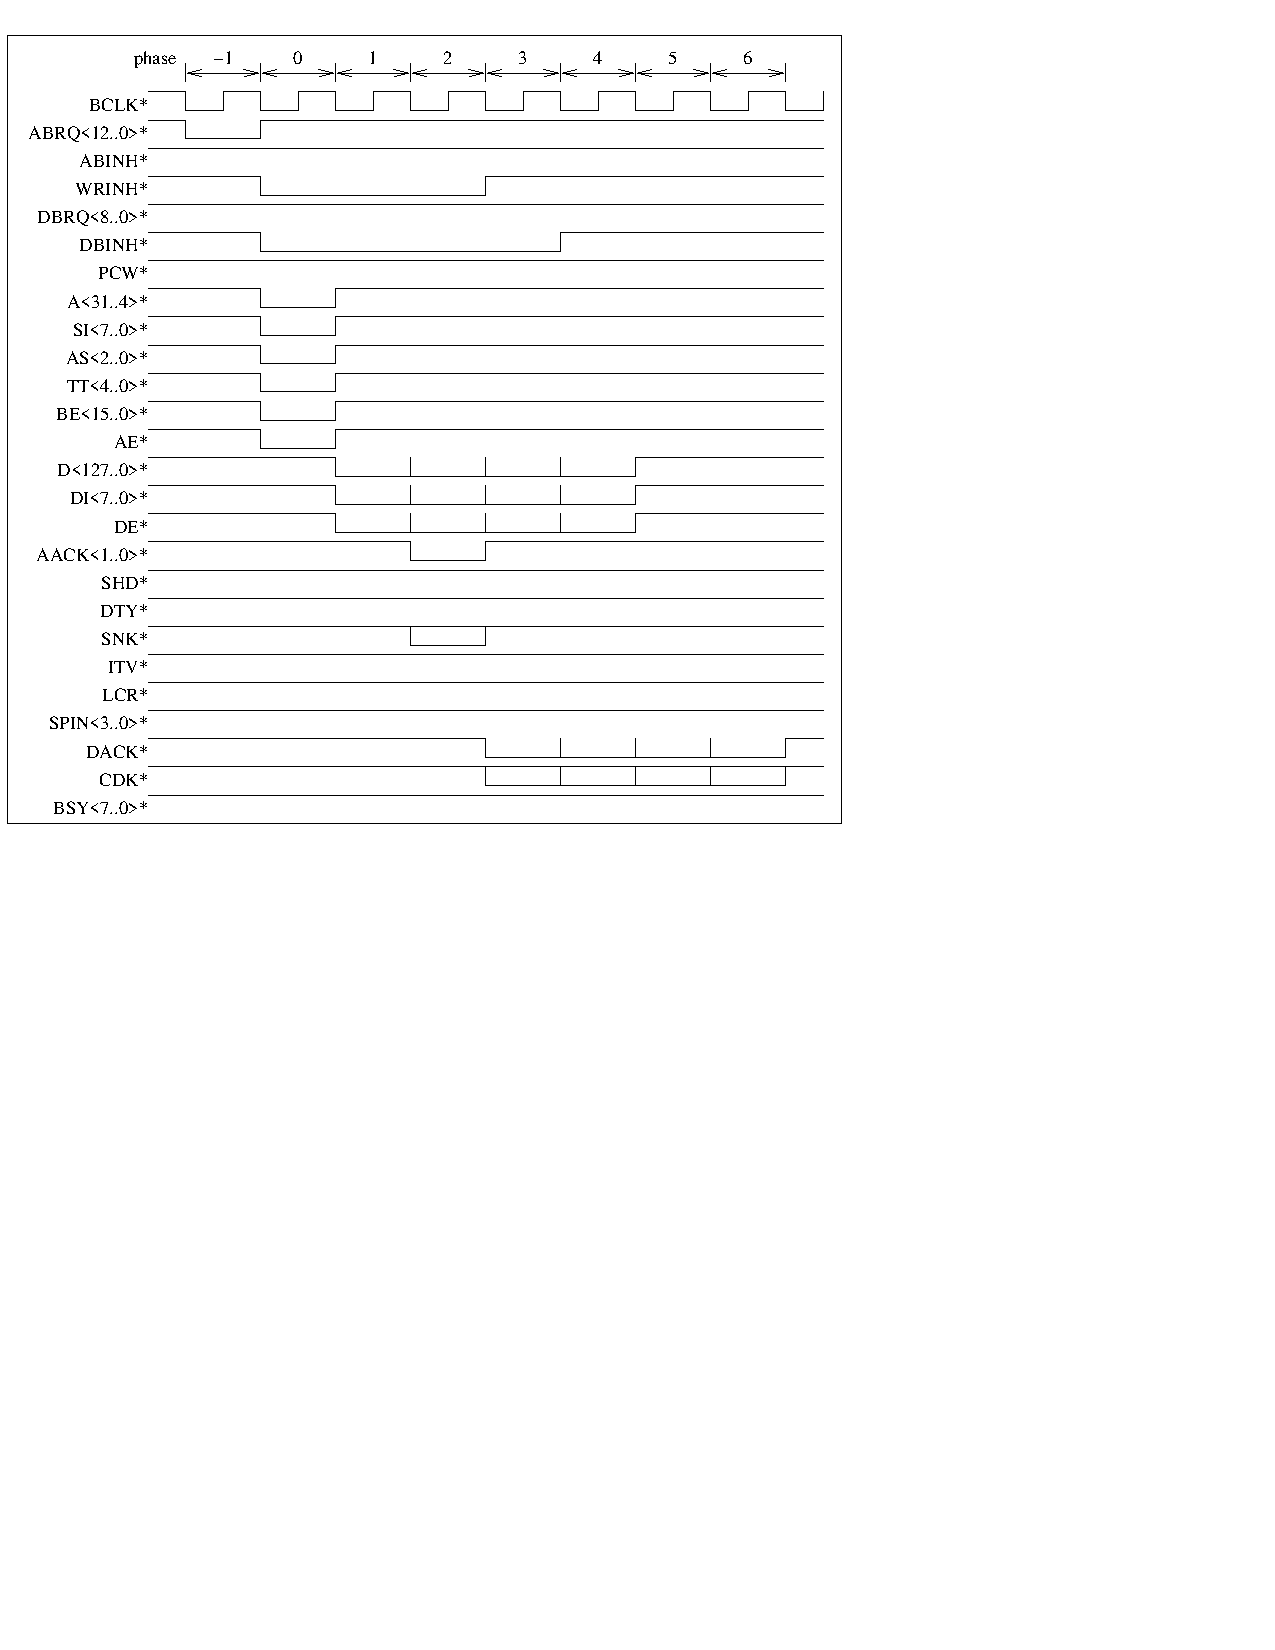
\includegraphics{ch3/FIG/block-add-data-basic.jpg}}
   \caption{블록 전송 어드레스 데이터 기본 사이클}\label{figure:block-add-data-basic}
\end{figure}
\begin{itemize}
	\item 블록 전송 어드레스 버스 중재 주기 - 단계 -1 (phase -1)\\
	어드레스 버스에 해당 어드레스를 구동하기에 앞서 수행하는 어드레스 버스 중재 동작.
	\item 블록 전송 어드레스 데이터 기본 주기 - 단계 0 (phase 0)\\
	중재 버스를 통하여 버스 사용허가를 받은 RQ가 한 버스 클럭 주기 동안 
	버스 상에 어드레스와 관련한 정보를 전송한다.
	32 비트의 어드레스, 어드레스 영역, 전송 형태, 바이트 마스크, RQ의 슬롯과
	채널 어드레스등과 각 신호의 패리티가 전송된다.
	이 주기 동안 사용되는 신호는 A$<$31..4$>$*, AP$<$3..0$>$*,
	AS$<$2..0$>$*, TT$<$4..0$>$*, STP*,
	BE$<$15..0$>$*, BEP$<$1..0$>$*,
	SI$<$7..0$>$*, SIP*, AE*등이다.
	RP들은 이 단계의 끝 부분에서 어드레스 버스에 실린 신호를 모두 저장한다. \\
	캐쉬를 갖는 RQ들도 이 단계의 끝 부분에서 어드레스 버스에 실린 신호를 모두 저장한다. \\
	다른 블록 전송 쓰기와의 데이터 충돌을 방지하기 위해 WRINH* 신호를 구동한다.
	다른 전송의 데이터와 충돌을 방지하기 위해 DBINH* 신호를 구동한다.
%
	\item 블록 전송 어드레스 데이터 기본 주기 - 단계 1 (phase 1)\\
	단계 0를 구동한 RQ가 계속해서 데이터 버스를 구동한다.
	이 단계에서 구동되는 신호선은 D$<$127..0$>$*,
	DP$<$15..0$>$*, DI$<$7..0$>$*, DIP*, DE*등이다.
	데이터 기본 주기와는 달리 별도의 데이터 중재 과정이 없다. \\
%	따라서 데이터 주기를 수행하고자 하는 RP와 충돌이 발생하지 않토록 데이터 중재기들은
%	어드레스 데이터 주기의 단계 1에서는 중재를 수행하지 않는다. \\
	RP들은 단계 0에서 저장한 어드레스 버스의 정보들의 에러 확인과 번역을 수행한다.
	또한 단계 1의 부분에서는 RQ로부터 오는 데이터를 저장한다. \\
	캐쉬를 갖는 RQ들은 캐쉬 동일성 유지를 위한 동작을 내부적으로 수행한다. \\
	다른 블록 전송 쓰기와의 데이터 충돌을 방지하기 위해 WRINH* 신호를 구동한다.
	다른 전송의 데이터와 충돌을 방지하기 위해 DBINH* 신호를 구동한다.
%
	\item 블록 전송 어드레스 데이터 기본 주기 - 단계 2 (phase 2)\\
	단계 2에서는 어드레스에 의해 선정된 한 RP가 단계 0에서 전송된 정보들에
	대한 응답을 버스 상에 구동하고 단계 1에서 받은 데이터의 패리티 에러를 확인한다.
	이때 사용되는 신호는 AACK$<$1..0$>$* 이고,
	만약 단계 0에서 전송된 정보에 에러가 검출될 경우 신호 구동과 데이터 패리티 확인을
	수행하지 않는다. \\
	단계 0를 구동한 RQ가 계속해서 데이터 버스를 구동한다.
	이 단계에서 구동되는 신호선은 D$<$127..0$>$*,
	DP$<$15..0$>$*, DI$<$7..0$>$*, DIP*, DE*등이다.
	데이터 기본 주기와는 달리 별도의 데이터 중재 과정이 없다. \\
	캐쉬를 갖는 RQ들이 단계 0에서 저장한 어드레스에 대한 
	캐쉬 동일성 유지 동작을 수행함에 있어서 문제가 발생하면 SNK* 신호를 구동한다.
	단계 0를 수행했던 RQ는 어드레스 상태 신호를 저장한다. \\
	다른 블록 전송 어드레스 데이터 기본주기와의 데이터 충돌을 방지하기 위해 WRINH* 신호를 구동한다.
	다른 전송의 데이터와 충돌을 방지하기 위해 DBINH* 신호를 구동한다.
%
	\item 블록 전송 어드레스 데이터 기본 주기 - 단계 3 (phase 3)\\
	단계 1에서 전송된 데이터를 받은 RP가 RQ로 응답하는 단계이다.
	데이터의 에러 유무를 보고한다. 이때 사용하는 신호선은 DACK*이다.
	그러나 현재 진행 중인 전송이 ITW인 경우 DACK*는 의미가 없고 대신 CDK*가 사용된다.
	단계 2의 응답에서 어드레스를 정상적으로 접수하지 못했다는 반응이 있었을 경우
	이 단계의 응답은 의미가 없다. \\
	단계 0를 구동한 RQ가 계속해서 데이터 버스를 구동한다.
	이 단계에서 구동되는 신호선은 D$<$127..0$>$*,
	DP$<$15..0$>$*, DI$<$7..0$>$*, DIP*, DE*등이다.
	데이터 기본 주기와는 달리 별도의 데이터 중재 과정이 없다. \\
	단계 0에 구동된 어드레스에 의해 선택된 RP는
	단계 1에 구동된 데이터에 대한 데이터 응답 DACK*을 구동하고,
	RQ는 해당 데이터 응답을 저장한다.
	그러나 현재 진행중인 전송이 ITW인 경우 DACK*는 의미가 없고 대신 CDK*가 사용된다.\\
	다른 전송의 데이터와 충돌을 방지하기 위해 DBINH* 신호를 구동한다.
%
	\item 블록 전송 어드레스 데이터 기본 주기 - 단계 4 (phase 4)\\
	단계 2에서 전송된 데이터를 받은 RP가 RQ로 응답하는 단계이다.
	데이터의 에러 유무를 보고한다. 이때 사용하는 신호선은 DACK* 이다.
	그러나 현재 진행 중인 전송이 ITW인 경우 DACK*는 의미가 없고 대신 CDK*가 사용된다.
	단계 2의 응답에서 어드레스를 정상적으로 접수하지 못했다는 반응이 있었을 경우
	이 단계의 응답은 의미가 없다. \\
	단계 0를 구동한 RQ가 계속해서 데이터 버스를 구동한다.
	이 단계에서 구동되는 신호선은 D$<$127..0$>$*,
	DP$<$15..0$>$*, DI$<$7..0$>$*, DIP*, DE*등이다.
	데이터 기본 주기와는 달리 별도의 데이터 중재 과정이 없다. \\
	단계 0에 구동된 어드레스에 의해 선택된 RP는
	단계 2에 구동된 데이터에 대한 데이터 응답을 구동하고, RQ는 해당 데이터 응답을 저장한다. \\
%
	\item 블록 전송 어드레스 데이터 기본 주기 - 단계 5 (phase 5)\\
	단계 3에서 전송된 데이터를 받은 RP가 RQ로 응답하는 단계이다.
	데이터의 에러 유무를 보고한다. 이때 사용하는 신호선은 DACK*이다.
	그러나 현재 진행중인 전송이 ITW인 경우 DACK*는 의미가 없고 대신 CDK*가 사용된다.
	단계 2의 응답에서 어드레스를 정상적으로 접수하지 못했다는 반응이 있었을 경우
	이 단계의 응답은 의미가 없다. \\
	단계 0에 구동된 어드레스에 의해 선택된 RP는
	단계 3에 구동된 데이터에 대한 데이터 응답을 구동하고, RQ는 해당 데이터 응답을 저장한다. \\
%
	\item 블록 전송 어드레스 데이터 기본 주기 - 단계 6 (phase 6)\\
	단계 4에서 전송된 데이터를 받은 RP가 RQ로 응답하는 단계이다.
	데이터의 에러 유무를 보고한다. 이때 사용하는 신호선은 DACK* 이다.
	그러나 현재 진행 중인 전송이 ITW인 경우 DACK*는 의미가 없고 대신 CDK*가 사용된다.
	단계 2의 응답에서 어드레스를 정상적으로 접수하지 못했다는 반응이 있었을 경우
	이 단계의 응답은 의미가 없다. \\
	단계 0에 구동된 어드레스에 의해 선택된 RP는
	단계 4에 구동된 데이터에 대한 데이터 응답을 구동하고, RQ는 해당 데이터 응답을 저장한다. \\
%
\end{itemize}
%
%
\subsection{전송의 구분}
정의된 전송의 종류는 NRD, NWR, NCR, NCW, IVD,
ILR, ILW, BRD, BWR, CRD, EXR, WRB, ITW로
13 가지이지만 실제 데이터가 이동되는 것은 IVD를 제외한 12 가지 전송형태이다.
그리고 데이터 이동이 수반되는 전송형태는 데이터의 실제 이동 방향에 따라
읽기 전송 모임(read transfer class)과 쓰기 전송 모임(write transfer class)으로 구분할 수 있다.
읽기 전송 모임은 데이터가 RP로부터 RQ로 이동하는 경우로써 NRD, NCR, CRD, EXR, BRD,
그리고 ILR가 여기에 속한다.
쓰기 전송 모임은 데이터가 RQ에서 RP로 이동하는 경우로써 NWR, NCW, WRB, BWR, 그리고 ILW가 여기에 속한다.
특히 ITW의 경우는 쓰기 전송과 비슷하지만 데이타는 RQ에서 RQ로 이동한다.
그리고 이동하는 데이터의 크기에 따라 단일 전송과 블록 전송으로 구분되며,
단일 전송의 경우 16바이트 이내의 연속된 데이터 전송에 사용되고,
블록 전송의 경우 64바이트 데이터 전송에 사용된다.
단일 전송에는 NRD, NWR, NCR, NCW, ILR, ILW가 있고,
블록 전송에는 BRD, BWR, CRD, EXR, WRB, ITW가 있다.
%
\subsubsection{단일 읽기 전송 모임}
단일 전송 읽기 전송은 단일 전송 어드레스 기본 사이클과 단일 전송 데이터 기본 사이클로 구성된다.
데이터가 필요한 RQ가 어드레스 기본 사이클을 수행하고, 어드레스 기본 사이클에 구동된 어드레스에 의해
선택된 RP는 단일 전송 데이터 기본 사이클을 수행하여 요청된 데이터를 전송하게 된다.
$<$그림~\ref{figure:single-read}$>$는 읽기 전송 모임의 진행 순서를 나타낸다.
%\input{ch3/TBL/read-class}
\begin{figure}[hp]
   \centerline{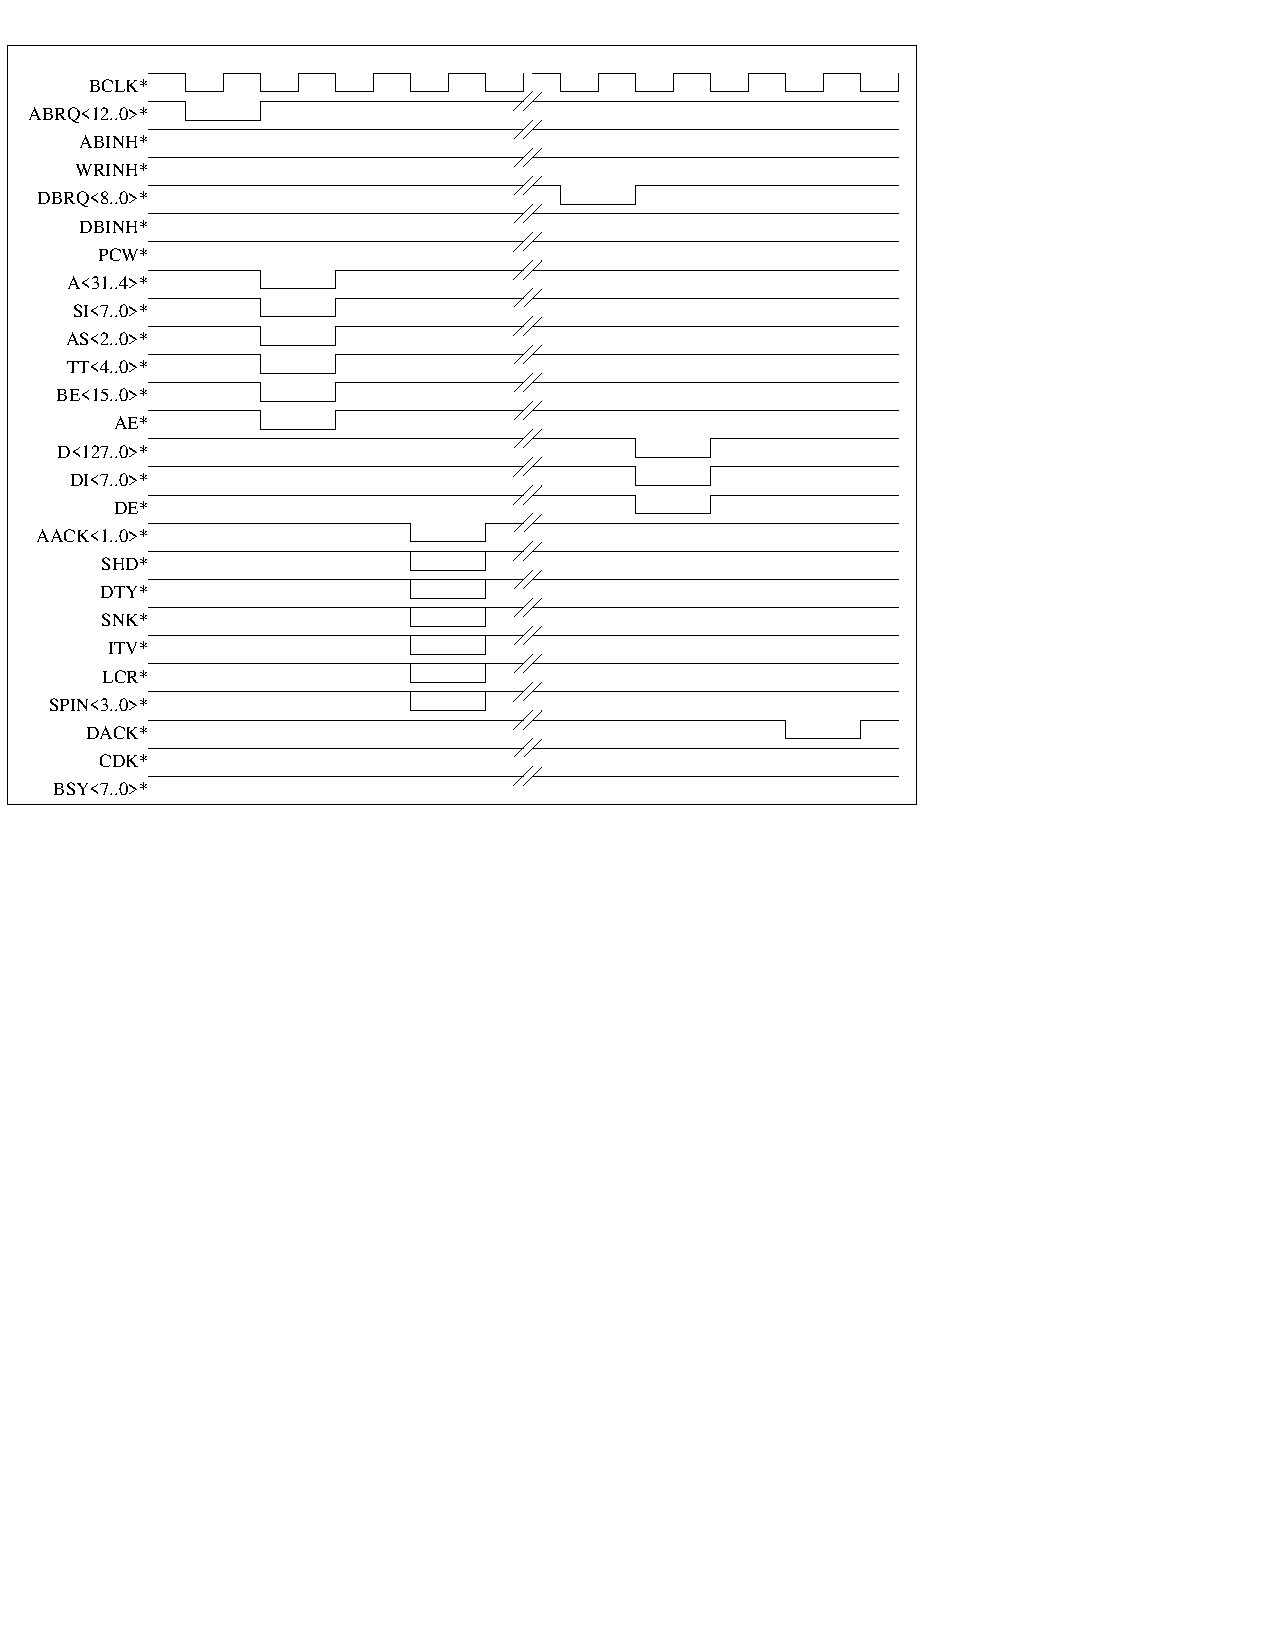
\includegraphics{ch3/FIG/single-read.jpg}}
   \caption{단일 읽기 전송}\label{figure:single-read}
\end{figure}
%
\subsubsection{단일 쓰기 전송 모임}
단일 전송 쓰기 전송은 단일 전송 어드레스 데이터 기본 사이클로 구성된다.
특정 RQ가 특정 RP로 데이터를 공급하는 전송이다.
$<$그림~\ref{figure:single-write}$>$는 쓰기 전송 모임의 진행 순서를 나타낸다.
%input{ch3/TBL/write-class}
\begin{figure}[hp]
   \centerline{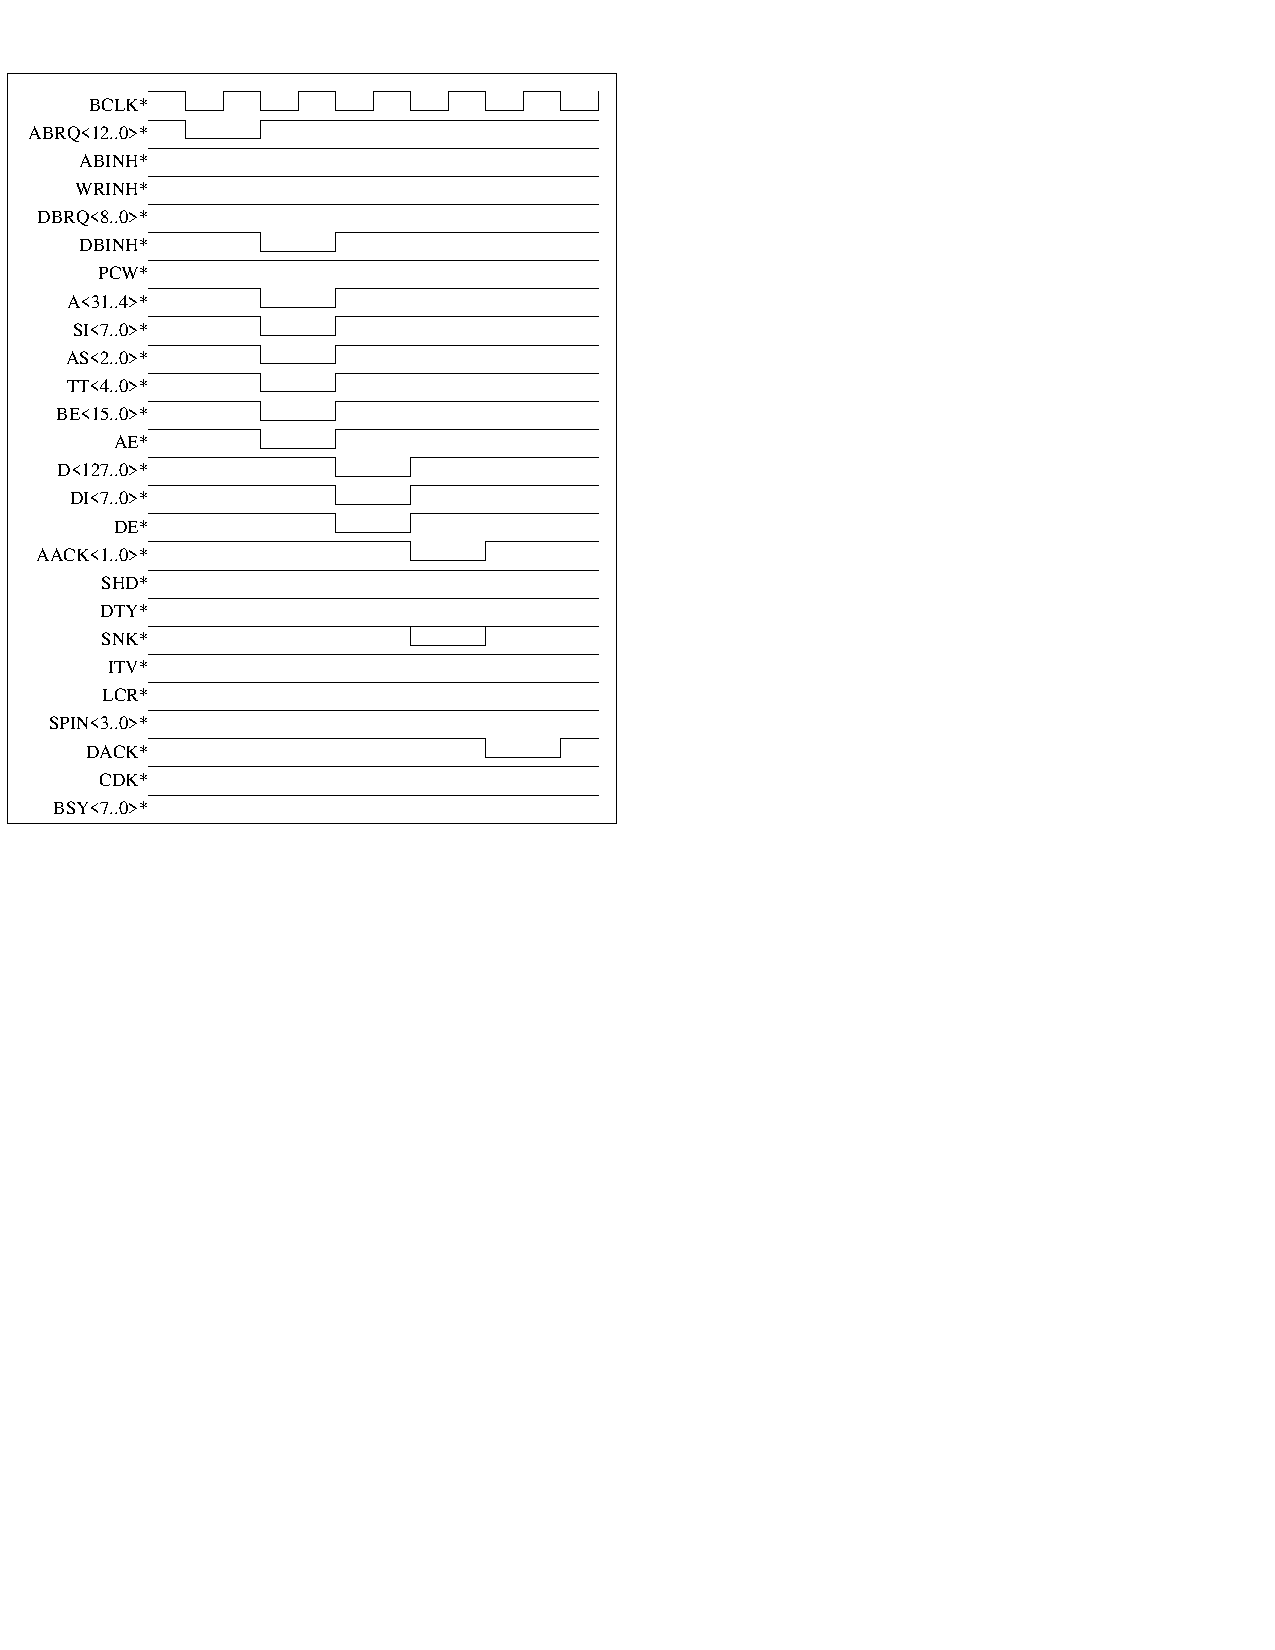
\includegraphics{ch3/FIG/single-write.jpg}}
   \caption{단일 쓰기 전송}\label{figure:single-write}
\end{figure}
%
\subsubsection{블록 읽기 전송 모임}
블록 전송 읽기 전송은 블록 전송 어드레스 기본 사이클과 블록 전송 데이터 기본 사이클로 구성된다.
데이터가 필요한 RQ가 어드레스 기본 사이클을 수행하고, 어드레스 기본 사이클에 구동된 어드레스에 의해
선택된 RP는 블록 전송 데이터 기본 사이클을 수행하여 요청된 데이터를 전송하게 된다.
\begin{figure}[hp]
   \centerline{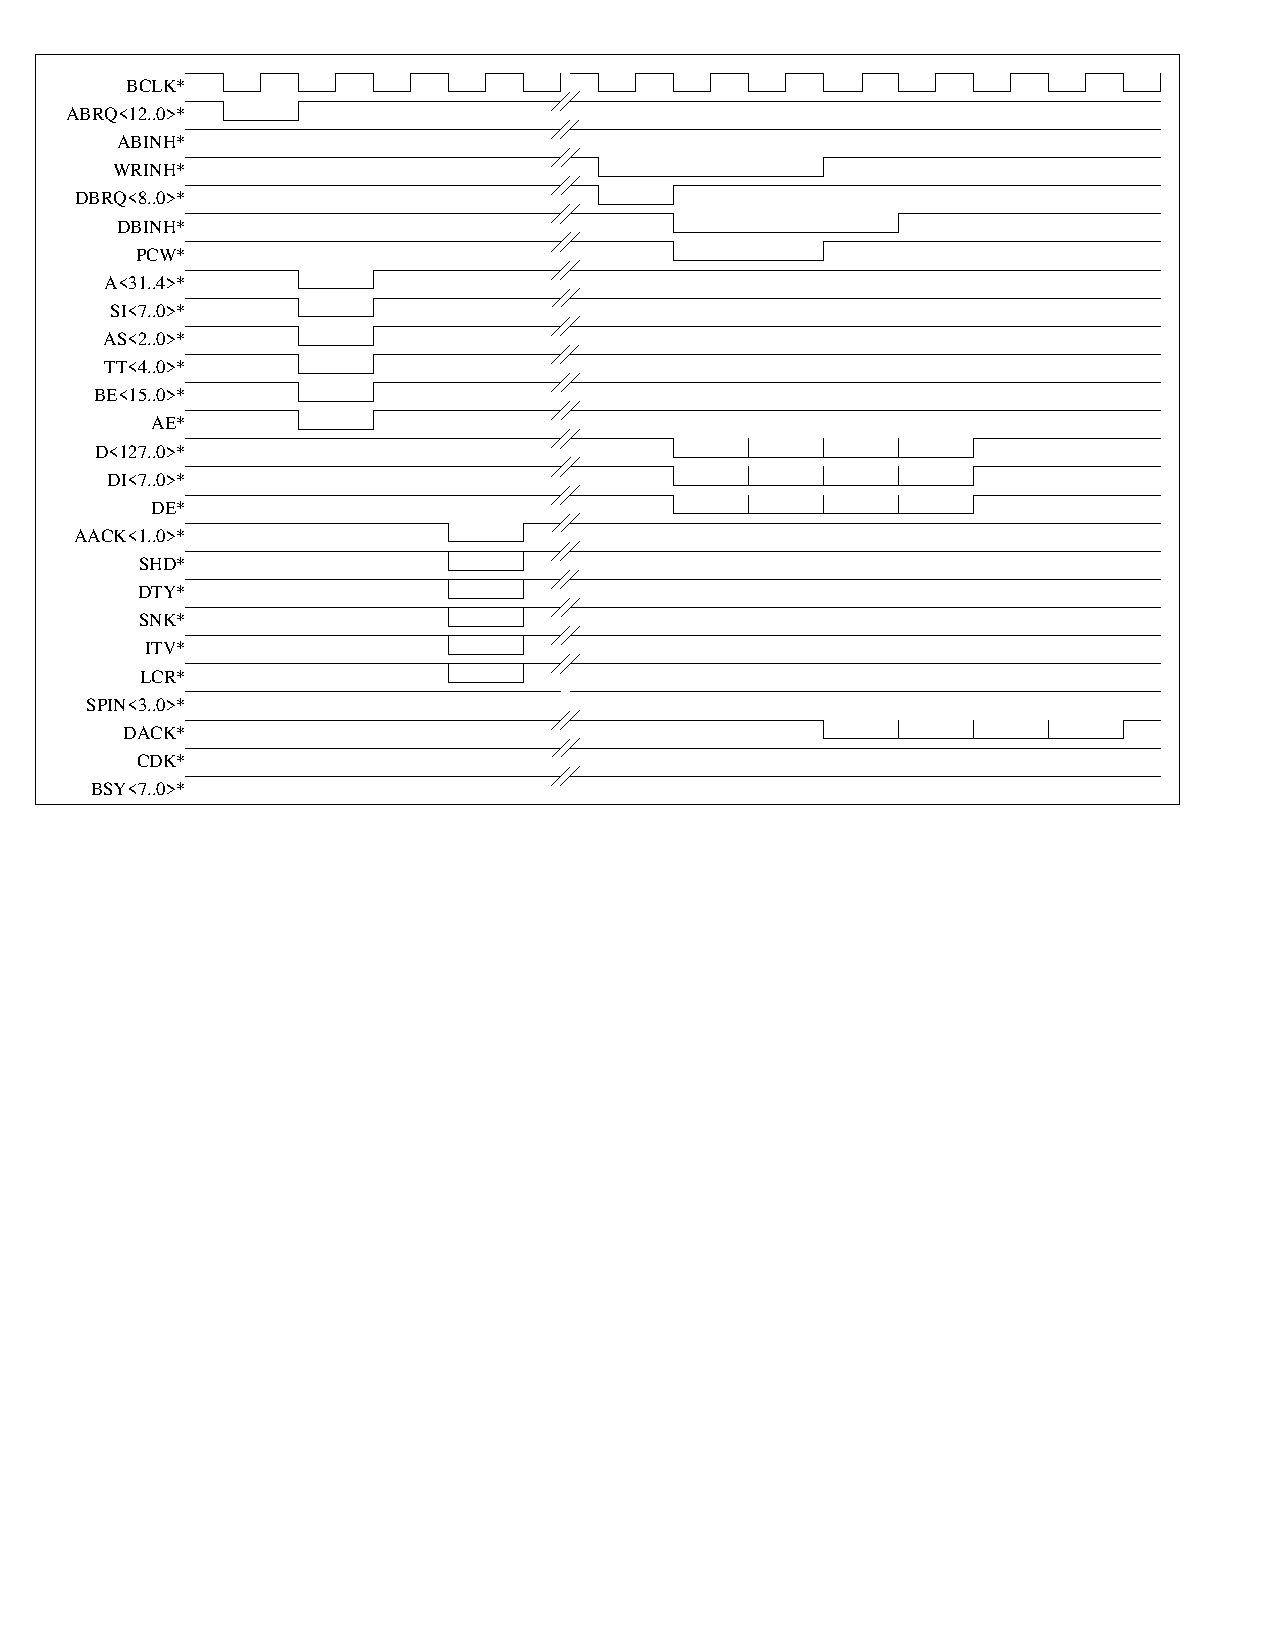
\includegraphics[angle=90]{ch3/FIG/block-read.jpg}}
   \caption{블록 읽기 전송}\label{figure:block-read}
\end{figure}
%
\subsubsection{블록 쓰기 전송 모임}
블록 전송 쓰기 전송은 블록 전송 어드레스 데이터 기본 사이클로 구성된다.
특정 RQ에서 특정 RP로, 혹은 특정 RQ에서 다른 특정 RQ로 데이터를 공급하는 전송이다.
\begin{figure}[hp]
   \centerline{\includegraphics{ch3/FIG/block-write.jpg}}
   \caption{블록 쓰기 전송}\label{figure:block-write}
\end{figure}
%%%%%
%\end{document}
%%%%%
